\documentclass[11pt]{article}
\usepackage[margin=3cm]{geometry}
\usepackage{algorithm2e}
\usepackage[italian]{babel}
\usepackage[hidelinks]{hyperref}
\usepackage{amsmath}
\usepackage{graphicx}
\usepackage[nameinlink, noabbrev, italian]{cleveref}

\tolerance=1
\emergencystretch=\maxdimen
\hyphenpenalty=10000
\hbadness=10000
\setlength\parindent{0pt}

\begin{document}
\begin{titlepage}
    \begin{center}
        \vspace*{5cm}
            
        \Huge
        \textbf{Cellular Connectivity and\\Noise Map}
            
        \vspace{0.5cm}
        \LARGE
        Relazione
            
        \vspace{1cm}
          
		\hfill
		\begin{center}
        	{\large{\bf Xia $\cdot$ Tian Cheng}}\\[-0.2em]
			{\large Matricola: \texttt{0000975129}}\\[-0.2em]
			{\large Email: tiancheng.xia@studio.unibo.it}
        \end{center}
            
        \vspace{4cm}
            
        Anno accademico\\
        $2022 - 2023$
            
        \vspace{0.8cm}
            
            
        \Large
        Corso di Laboratorio di applicazioni mobili\\
        Alma Mater Studiorum $\cdot$ Università di Bologna\\
            
    \end{center}
\end{titlepage}
\newpage

\pagenumbering{roman}
\tableofcontents
\newpage

\pagenumbering{arabic}


\section{Introduzione}

\subsection{Feature implementate}




\section{Scelte progettuali}

\subsection{Informazioni generali}



\subsection{Mappa}
Per la mappa è stato utilizzato \textit{Google Maps} e l'implementazione è contenuta nel fragment \texttt{WaveHeatMapFragment}.

\subsubsection{Generazione cella}
Una cella della mappa rappresenta la misurazione di un'area quadrata\footnote{Esclusa la zona equatoriale, le celle appariranno rettangolari} e la dimensione di quest'ultima scala automaticamente in base al livello dello zoom.

Una cella è descritta dalle coordinate del vertice superiore sinistro (nord-ovest) e a partire da questa vengono calcolate le coordinate degli altri convertendo la dimensione della cella (in metri) in un offset da applicare a latitudine e longitudine.

Per questioni estetiche, gli offset applicati alle coordinate sono approssimati in modo tale che tutte le righe siano allineate verticalmente (vedi \cref{fig:tile_offset}).
\begin{figure}[h]
    \centering
    \begin{minipage}[b]{0.45\textwidth}
      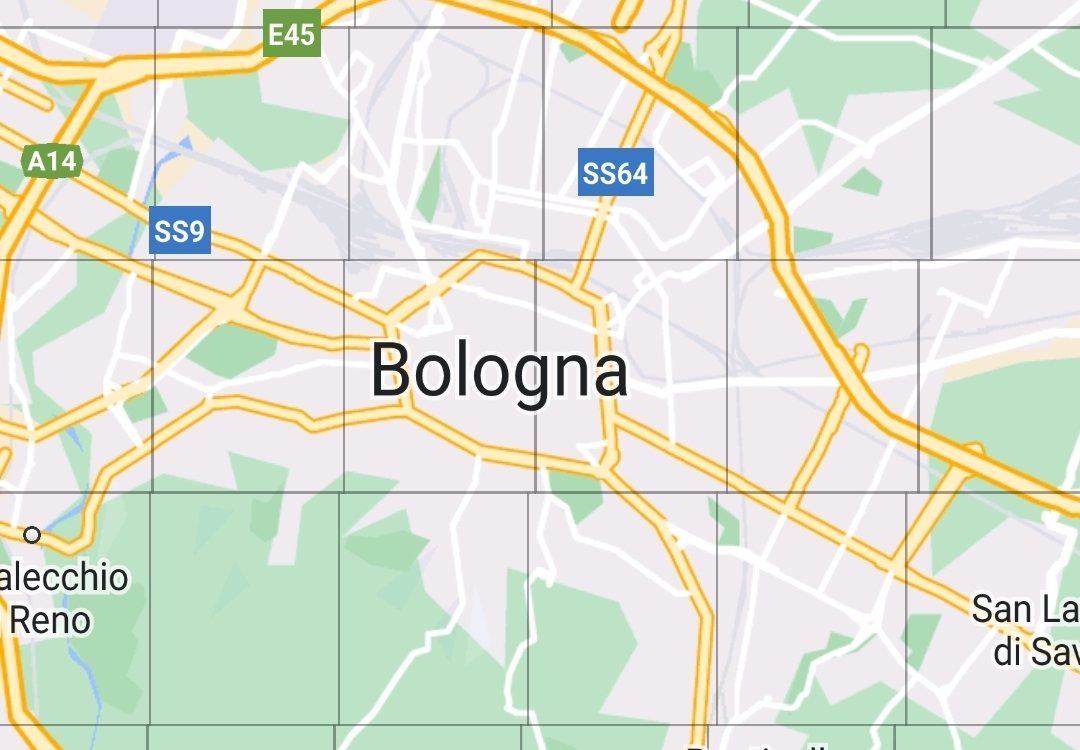
\includegraphics[width=\textwidth]{./img/tile_no_approx.jpg}
    \end{minipage}
    \hfill
    \begin{minipage}[b]{0.45\textwidth}
      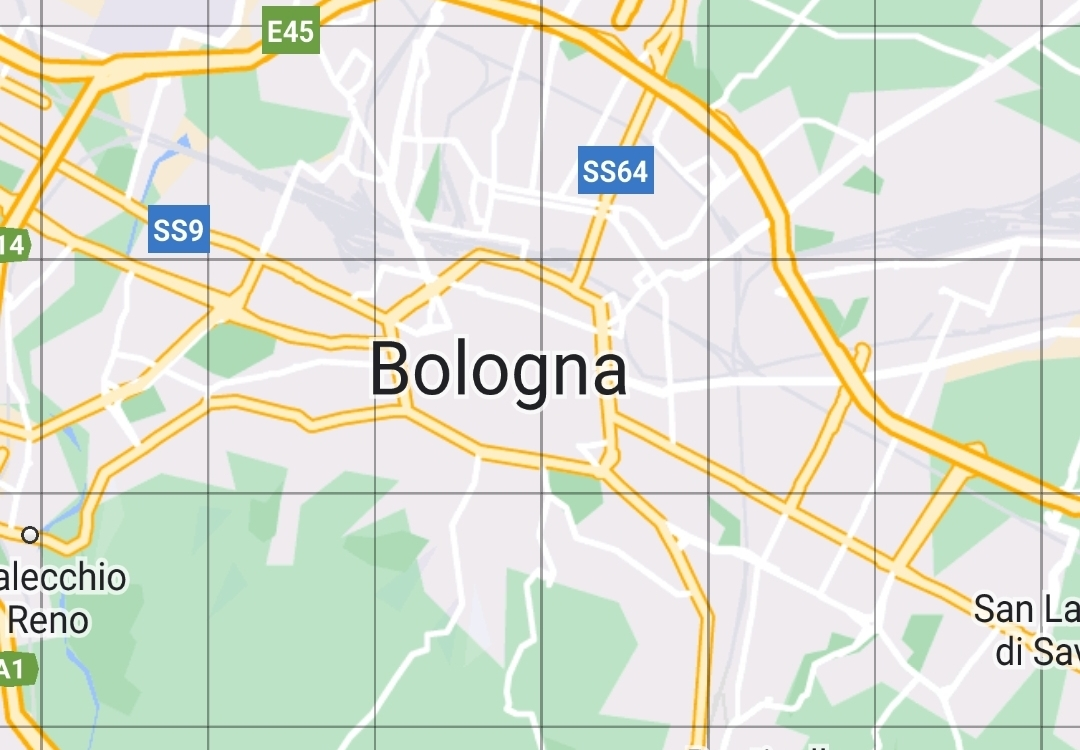
\includegraphics[width=\textwidth]{./img/tile_approx.jpg}
    \end{minipage}
    \caption{Offset calcolati in maniera precisa (sinistra) e approssimato (destra)} \label{fig:tile_offset}
\end{figure}

\subsubsection{Generazione griglia}
La griglia è composta da celle generate relativamente ad una posizione di riferimento. In particolare, in fase di inizializzazione viene designata come cella di riferimento quella che pone la posizione dell'utente al centro e in base a questa è possibile determinare la posizione di tutte le altre celle della mappa. 

Nello specifico, date delle coordinate $(\texttt{pos}_{\texttt{lat}}, \texttt{pos}_{\texttt{lon}})$, per determinare la cella che la contiene si calcola il numero di celle da saltare rispetto a quella di riferimento: 
\begin{equation*}
    \texttt{to\_skip\_tiles}_\texttt{lat} =
        \lceil \frac{\texttt{pos}_{\texttt{lat}} - \texttt{center\_top\_left}_{\texttt{lat}}}{\texttt{latitudeOffset(tile\_length\_meters)}} \rceil
\end{equation*}
\begin{equation*}
    \texttt{to\_skip\_tiles}_\texttt{lon} =
        \lfloor \frac{\texttt{pos}_{\texttt{lon}} - \texttt{center\_top\_left}_{\texttt{lon}}}{\texttt{longitudeOffset(tile\_length\_meters)}} \rfloor
\end{equation*}
Le coordinate del vertice superiore sinistro sono quindi:
\begin{equation*}
    \texttt{tile}_\texttt{lat} = \texttt{center\_top\_left}_{\texttt{lat}} + (\texttt{to\_skip\_tiles}_\texttt{lat} \cdot \texttt{latitudeOffset(tile\_length\_meters)})
\end{equation*}
\begin{equation*}
    \texttt{tile}_\texttt{lon} = \texttt{center\_top\_left}_{\texttt{lon}} + (\texttt{to\_skip\_tiles}_\texttt{lon} \cdot \texttt{longitudeOffset(tile\_length\_meters)})
\end{equation*}

Con questo approccio, ogni volta che viene spostata la visuale della mappa, la griglia viene generata iterando a partire dalle coordinate dell'angolo nord-ovest visibile dello schermo, fino a raggiungere l'angolo sud-est. 

In aggiunta, per maggiore efficienza, si tiene traccia delle celle generate in modo da evitare di ridisegnare una cella già presente. Questo meccanismo viene resettato quando viene cambiato il livello di zoom, in quanto tutte le celle già presenti diventano obsolete e vengono cancellate.

\subsection{Raccolta dei dati}

\subsubsection{Struttura e memorizzazione delle misurazioni}
Una misurazione è descritta dall'interfaccia \texttt{WaveMeasure} e contiene il valore della misurazione, un timestamp, la posizione e un flag per indicare se si tratta di una misurazione propria o ottenuta tramite condivisione. 
In aggiunta, è presente un campo per informazioni aggiuntive utile per distinguere alcune tipologie di misurazioni (es. per Wi-Fi e Bluetooth viene salvato il BSSID).

L'interfaccia \texttt{WaveMeasure} viene quindi utilizzata per implementare la classe \texttt{MeasureTable} che descrive la tabella del database dedicata per memorizzare le misurazioni. 
Tutte le misurazioni sono salvate nella stessa tabella e sono differenziate da un campo \texttt{type}.


\subsubsection{Sampler}
Per la raccolta dei dati è stato introdotto il concetto di \textit{sampler} per gestisce in maniera modulare le misurazioni.
Nello specifico, un \textit{sampler} è descritto dalla classe astratta \texttt{WaveSampler} e richiede l'implementazione dei seguenti metodi:
\begin{itemize}
    \item \texttt{sample} per prendere una nuova misurazione
    \item \texttt{store} per il salvataggio dei dati nel database
    \item \texttt{retrieve} per la ricerca dei dati note le coordinate dei vertici di una cella della mappa
\end{itemize}
Inoltre, sono esposte le seguenti funzioni ausiliarie:
\begin{itemize}
    \item \texttt{average} richiama \texttt{retrieve} e restituisce la media dei valori
    \item \texttt{sampleAndStore} richiama in sequenza \texttt{sample} e \texttt{store}
\end{itemize}
Per maggiore flessibilità, le misure vengono sempre intese come liste di \texttt{WaveMeasure}. Ciò permette di gestire misurazioni che per loro natura non generano un'unica misurazione (es. Wi-Fi e Bluetooth).

A partire da \texttt{WaveSampler} sono quindi implementati i \textit{sampler} per Wi-Fi, Bluetooth, LTE e suono.


\subsection{Servizi in background}


\subsection{Condivisione dati}


\section{Criticità e problemi noti}

\end{document}
